\begin{frame}
	\frametitle{branches}

	\begin{block}{}
		\begin{itemize}
			\item point to a commit (flat file with sha1 hash).
			\item moves pointer on commit, revert, rebase, reset, ...
			\item stored in .git/refs/
		\end{itemize}
	\end{block}
\end{frame}

\begin{frame}
	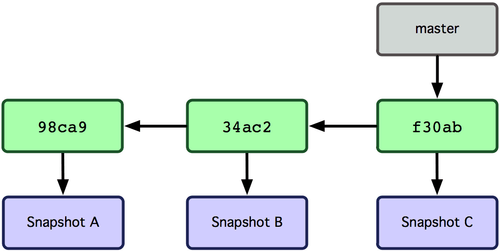
\includegraphics[width=\textwidth]{images/branches.png}
\end{frame}

\begin{frame}
	\frametitle{What is HEAD}

	\begin{block}{}
		\begin{itemize}
			\item points to a branch
			\item flat file with relative path to branch
			\item or sha1 hash in detached head mode.
			\item moves on git checkout
			\item does NOT move on revert, rebase, reset, commit, ...
		\end{itemize}
		\note[itemize]{
			\item `\$ git checkout head~ && cat .git/HEAD` (detached)
		}
	\end{block}
\end{frame}

\begin{frame}
	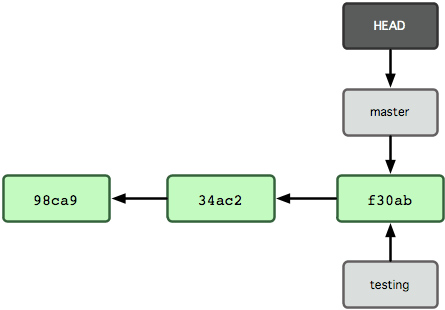
\includegraphics[width=\textwidth]{images/head.png}
\end{frame}

